\documentclass{jib}
\newlength{\platz}
\setlength{\platz}{15pt}
\RequirePackage{listings}

%\usepackage{changepage} %test, TODO remove

\lstset{%
  basicstyle=\ttfamily,
  fontadjust,
  flexiblecolumns=true,
  frame=L,
  xleftmargin=15pt,
  framesep=5pt,
  emphstyle=\rmfamily\itshape}
  

\usepackage{pdfpages}

%%%%%%%%%%%%%%%%%%%%%%%%%%%%%%%%%%%%%%%%%%%%%%%%%%%%%%%%%%
% JIB Header/Footer
%%%%%%%%%%%%%%%%%%%%%%%%%%%%%%%%%%%%%%%%%%%%%%%%%%%%%%%%%%
\jibvolume{XX} % insert volume
\jibissue{X}   % insert issue
\jibpages{XXX} % insert article ID
\jibyear{XXXX} % insert year
\makeHeaderFooter{} % leave as is
%%%%%%%%%%%%%%%%%%%%%%%%%%%%%%%%%%%%%%%%%%%%%%%%%%%%%%%%%%

\begin{document}

%%%%%%%%%%%%%%%%%%%%%%%%%%%%%%%%%%%%%%%%%%%%%%%%%%%%%%%%%%
%
% Title Page
%
%%%%%%%%%%%%%%%%%%%%%%%%%%%%%%%%%%%%%%%%%%%%%%%%%%%%%%%%%%

\begin{jibtitlepage}

\jibtitle{Synthetic Biology Open Language Visual (SBOL Visual) \\ Version 2.0}


%We did not provide author(s) nor author footnote(s), please complete as applicable.
% Please make sure to use unique footnote characters for each author
\jibauthor{Robert Sidney Cox\iref{kobe},
Curtis Madsen\iref{bu},
James McLaughlin\iref{newcastle},
Tramy Nguyen\iref{utah}, 
Nicholas Roehner\iref{bbn}, 
Bryan Bartley\iref{uw}, 
Swapnil Bhatia\iref{bu}, 
Mike Bissell\iref{amyris},  
Kevin Clancy\iref{thermo}, 
Thomas Gorochowski\iref{bristol}, 
Raik Grunberg\iref{kaust},
Augustin Luna\iref{harvard}, 
Nicolas Le Novere\iref{babraham}, 
Matthew Pocock\iref{turing}, 
Herbert Sauro\iref{uw}, 
John T. Sexton\iref{rice}, 
Guy-Bart Stan\iref{imperial}, 
Jeffrey J. Tabor\iref{rice}, 
Christopher A. Voigt\iref{mit}, 
Zach Zundel\iref{utah}, 
Chris Myers\iref{utah}, 
Jacob Beal\iref{bbn},
Anil Wipat\iref{newcastle}\jibauthorfootnote{*}{Correspondence should be addressed to:
           \email{editors@sbolstandard.org}}}

\addjibinstitution{kobe}{Kobe University, Japan}
\addjibinstitution{bu}{Boston University, USA}
\addjibinstitution{newcastle}{Newcastle University, UK}
\addjibinstitution{utah}{University of Utah, USA}
\addjibinstitution{bbn}{Raytheon BBN Technologies, USA}
\addjibinstitution{uw}{University of Washington, USA}
\addjibinstitution{amyris}{Amyris, Inc., USA}
\addjibinstitution{thermo}{Thermo Fisher Scientific, USA}
\addjibinstitution{bristol}{University of Bristol, UK}
\addjibinstitution{kaust}{KAUST, Saudi Arabia}
\addjibinstitution{harvard}{Harvard Medical School, USA}
\addjibinstitution{babraham}{Babraham Institute, UK}
\addjibinstitution{turing}{Turing Ate My Hamster, Ltd., UK}
\addjibinstitution{rice}{Rice University, USA}
\addjibinstitution{imperial}{Imperial College, UK}
\addjibinstitution{mit}{MIT, USA}


\end{jibtitlepage}


\begin{abstract}

People who are engineering biological organisms often find it useful to communicate in
diagrams, both about the structure of the nucleic acid sequences that they are engineering 
and about the functional relationships between sequence features and other molecular species.
%
Some typical practices and conventions have begun to emerge for such
diagrams.  The Synthetic Biology Open Language Visual (SBOL Visual) has been developed as a standard 
for organizing and systematizing such
conventions in order to produce a coherent language for expressing
the structure and function 
of genetic designs. 
%
This document details version 2.0 of SBOL Visual, which builds on the prior SBOL Visual 1.0 standard by
expanding diagram syntax to include functional interactions and molecular species, 
making the relationship between diagrams and the SBOL data model explicit, 
supporting families of symbol variants, 
clarifying a number of requirements and best practices,
and significantly expanding the collection of diagram glyphs.
\end{abstract}

% Include your PDF document
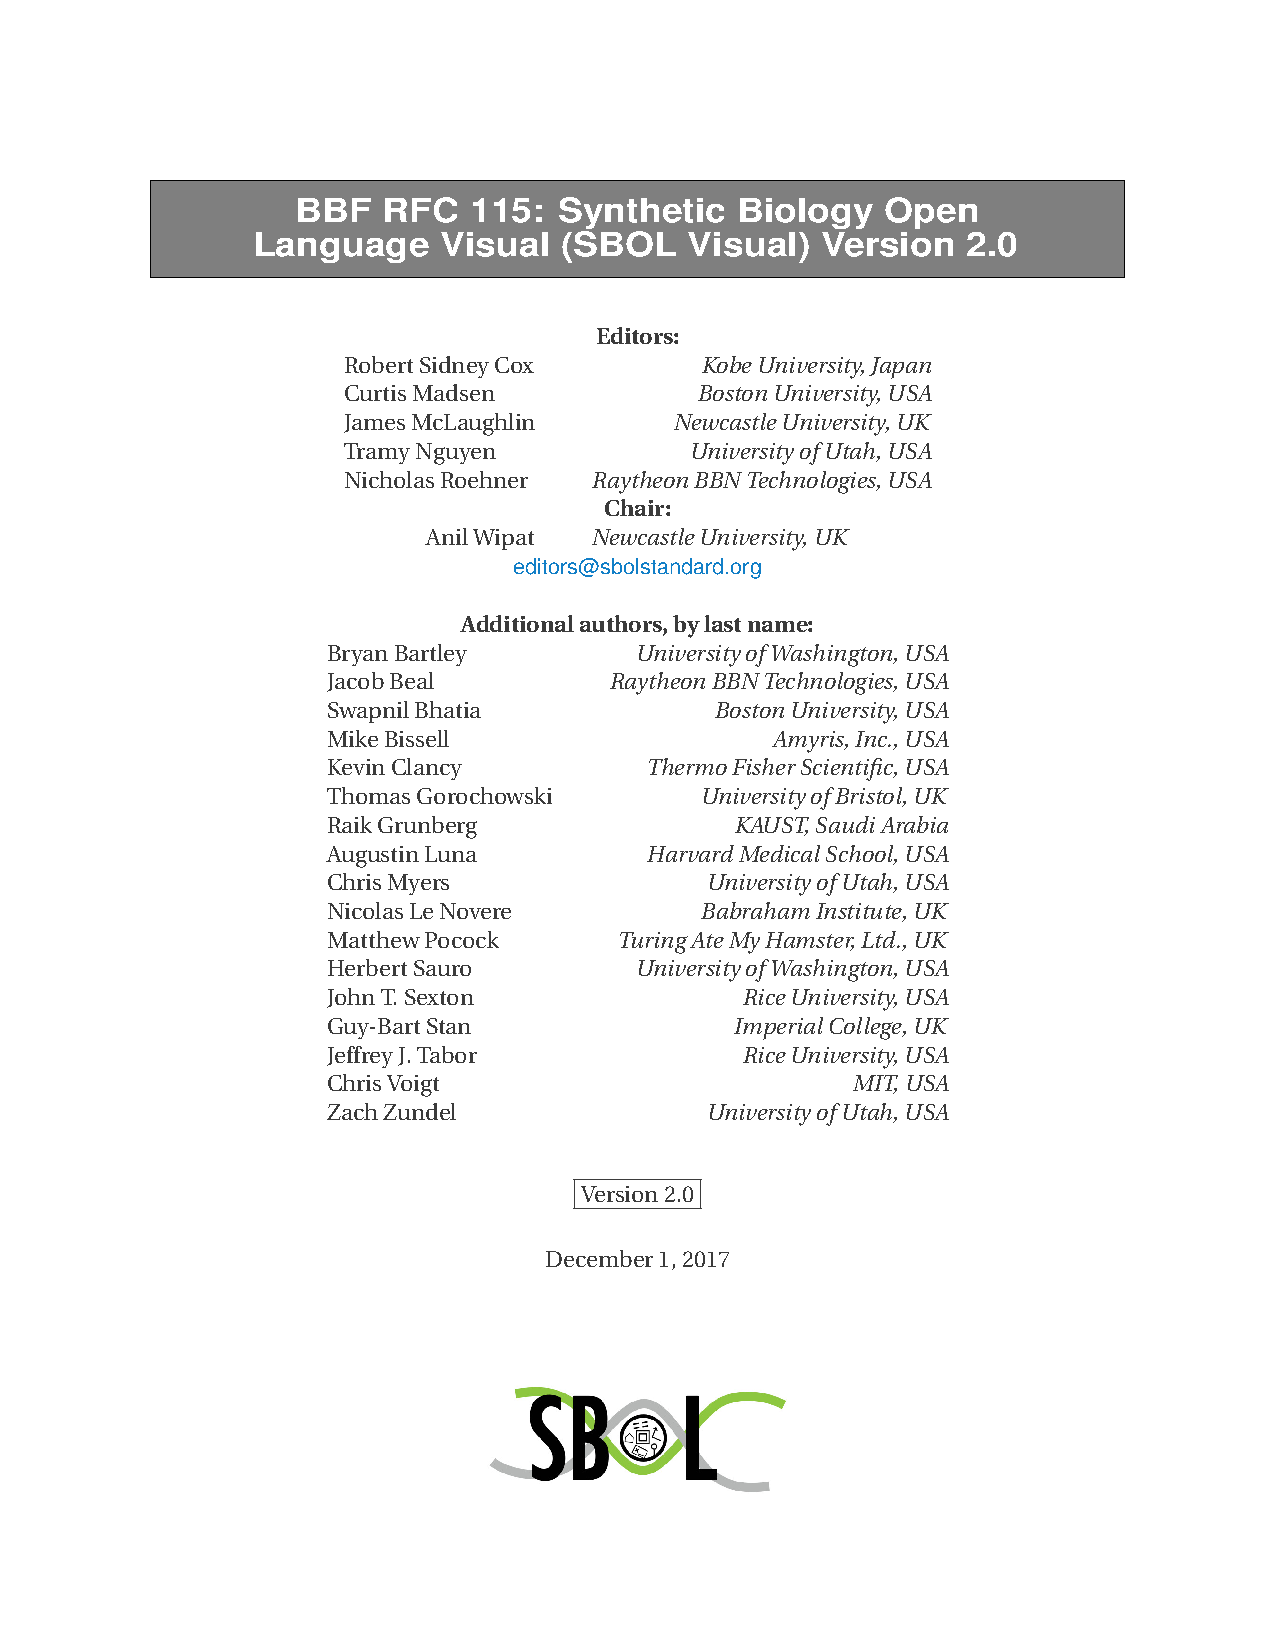
\includepdf[pages=-, offset=80 -80]{BBFRFC115_SBOL_Visual_2_0.pdf}

\end{document}
